\section{Программная реализация}

После изучения алгоритма Тарского была начата работа по реализации этого алгоритма, но не для произвольных формул, а для формул без параметров.

\begin{definition}
    Формула $\mathcal{A}$ называется \textbf{формулой без параметров}, если для любой ее подформулы вида $(Qx)\mathcal{B}$, формула $\mathcal{B}$ свободна от вхождений кванторов и от переменных, возможно, за исключением переменной $x$.
\end{definition}

Для этого были выбраны язык C\#, платформа .NET Core 3.1 и спецификация .NET Standard 2.1 \cite{TroelsonNet}. Такой выбор обусловлен рядом причин:
\begin{itemize}
    \item Язык C\#~--- это объектно-ориентированный язык программирования, а данная парадигма программирования позволяет абстрактно описывать объекты, в том числе и математические объекты; 
    \item .NET Core и .NET Standard~--- это современные, развивающиеся и востребованные кроссплатформенные технологии с открытым исходным кодом;
    \item Личные предпочтения автора.
\end{itemize}
Для поэтапного создания программы, были сформулированы и решены следующие задачи:
\begin{itemize}
    \item Разработать библиотеку классов для объектов языка элементарной алгебры: символы алфавита, термы, формулы;
    \item Реализовать ввод логических формул;
    \item Разработать библиотеку классов для рациональных чисел и многочленов от одной вещественной переменной с рациональными коэффициентами;
    \item Реализовать алгоритм Тарского для формул от одной переменной;
    \item Реализовать алгоритм элиминации кванторов (утверждение \ref{algB}) для формул без параметров;
    \item Обеспечить минимальное покрытие юнит-тестами;
    \item Собрать все библиотеки и модули в единый программный комплекс.
\end{itemize}
Написание программы осуществлялось в среде разработки Microsoft Visual Studio 2019 Community с установленным дополнением ReSharper. Обе программы доступны по специальным студенческим лицензиям для использования в некоммерческих целях.

\subsection{Представление формул}

Необходимо было начать с того, что создать абстракции для всех объектов языка элементарной алгебры: символы алфавита, термы, формулы. Для этого была написана библиотека классов LogicLanguageLib, в которой определены три пространства имён:
\begin{itemize}
    \item в LogicLanguageLib.Alphabet расположены классы для символов алфавита;
    \item в LogicLanguageLib.Words~--- классы для термов и формул языка;
    \item в LogicLanguageLib.IO~--- класс, решающий задачи системы ввода.
\end{itemize}

\subsubsection{Класс Symbol}

\begin{wrapfigure}{r}{0.21\textwidth}
    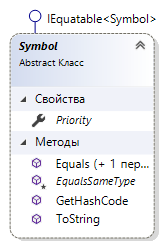
\includegraphics[width=0.9\linewidth]{Symbol.png} 
    \caption{}
    \label{fig:Symbol}
\end{wrapfigure}

Начнём с класса Symbol (рис. \ref{fig:Symbol})~--- это абстрактный класс, реализующий интерфейс IEquatable<Symbol>. Все классы для символов алфавита языка элементарной алгебры наследники этого класса, то есть класс Symbol~--- это базовый класс. 

Отдельно стоит отметить абстрактное свойство Priority, которое доступно только для чтения. Оно будет использоваться при построении обратной польской записи алгоритмом Дейкстры.

Методы ToString, GetHashCode и EqualsSameType тоже объявлены как абстрактные. Первые два~--- это стандартные методы для всех объектов, а последний вызывается при сравнении объектов, в методе Equals, когда известно, что сравниваемые объекты являются объектами одного типа.

Прямыми наследниками класса Symbol являются два абстрактных класса~--- LogicalSymbol и NonLogicalSymbol (рис. \ref{fig:Symbol-inh}), которые описывают логические и нелогические символы соответственно. Оба класса не содержат ни методов, ни свойств, но без них иерархия классов была бы неполной.

\begin{figure}[h]
    \center{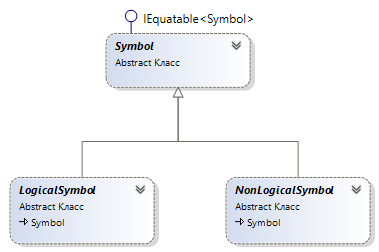
\includegraphics[width=0.6\linewidth]{Symbol-inh.png}}
    \caption{Фрагмент диаграммы классов.}
    \label{fig:Symbol-inh}
\end{figure}

Далее будут рассмотрены классы для логических символов (рис. \ref{fig:LogicalSymbol}) и для нелогических символов (рис. \ref{fig:NonLogicalSymbol}).

\begin{figure}[h]
    \center{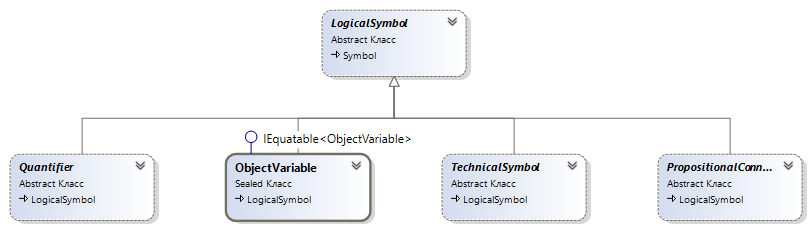
\includegraphics[width=1\linewidth]{Logical.png}}
    \caption{Фрагмент диаграммы классов.}
    \label{fig:LogicalSymbol}
\end{figure}

\begin{figure}[ht]
    \center{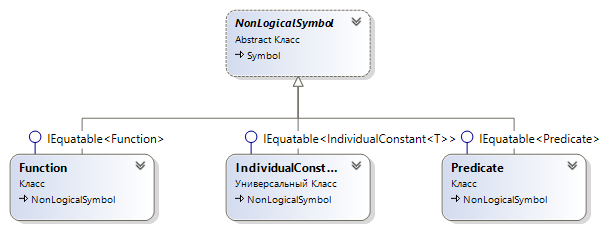
\includegraphics[width=0.8\linewidth]{NonLogical.png}}
    \caption{Фрагмент диаграммы классов.}
    \label{fig:NonLogicalSymbol}
\end{figure}

\subsubsection{Класс Quantifier}

\begin{wrapfigure}{r}{0.20\textwidth}
    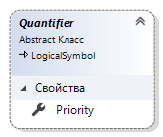
\includegraphics[width=0.9\linewidth]{Quantifier.png} 
    \caption{}
    \label{fig:Quantifier}
\end{wrapfigure}

Класс Quantifier (рис. \ref{fig:Quantifier}) создан для представления кванторов. Он не содержит никаких специальных методов или свойств, а только лишь реализует свойство Priority~--- всем кванторам присвоен приоритет 60. Кванторы всеобщности и существования описаны классами производными от класса Quantifier (рис. \ref{fig:Quantifier-inh}), притом оба класса реализуют паттерн одиночка, что достаточно естественно. Оба класса реализуют метод ToString~--- метод возвращает строку <<$\forall$>> или <<$\exists$>> соответственно.

\begin{figure}[h]
    \center{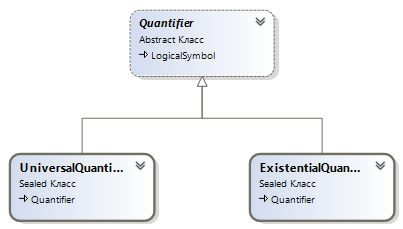
\includegraphics[width=0.4\linewidth]{Quantifier-inh.png}}
    \caption{Фрагмент диаграммы классов.}
    \label{fig:Quantifier-inh}
\end{figure}


\subsubsection{Класс ObjectVariable}

\begin{wrapfigure}{r}{0.24\textwidth}
    \vspace{-1.5cm}
    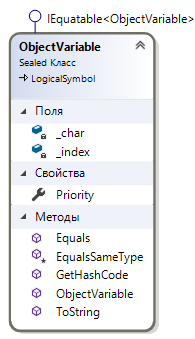
\includegraphics[width=0.9\linewidth]{ObjectVariable.png} 
    \vspace{-0.3cm}
    \caption{}
    \label{fig:ObjectVariable}
\end{wrapfigure}

Для индивидных (предметных) переменных написан класс ObjectVariable (рис. \ref{fig:ObjectVariable}). Класс реализует интерфейс IEquatable<ObjectVariable>. Каждая переменная~--- это буква и, возможно, индекс в виде числа. Например, $x$ и $A_1$~--- это переменные, а $xx$, $a1$, $t_i$ таковыми не являются. Поэтому при создании объекта происходят соответствующие проверки. И две переменные считаются равными, если равны их буквы и индексы.

Приоритет, то есть свойство Priority, для предметных переменных равен $-10$. А метод ToString, например, для переменной $x_1$ вернет строку <<$x\_ 1$>>. 

\subsubsection{Класс TechnicalSymbol}

Абстрактный класс TechnicalSymbol не содержит ни одного члена класса, но он является базовым для классов Comma, LeftBracket и RightBracket~--- запятая, левая и правая скобка соответственно. Классы-наследники вновь реализуют шаблон проектирования одиночка. Приоритет левой скобки равен $0$, а правой скобки и запятой равен $10$.

\begin{figure}[h]
    \center{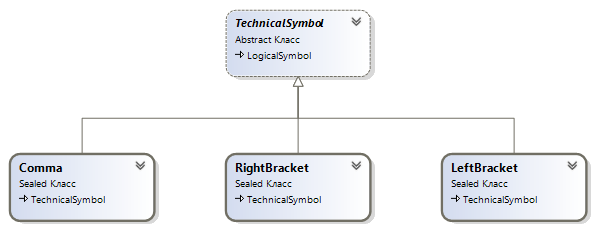
\includegraphics[width=0.6\linewidth]{TechnicalSymbol.png}}
    \caption{Фрагмент диаграммы классов.}
    \label{fig:TechnicalSymbol}
\end{figure}

\subsubsection{Класс PropositionalConnective}

Эта часть практически полностью взята из предыдущей работы \cite{Gibadulin1}, в которой также необходимо было реализовать представление формул, но формул исчисления высказываний. 

В абстрактном классе PropositionalConnective (рис. \ref{fig:PropositionalConnective}) определено поле Arity, то есть арность логической связки.

\begin{figure}[h]
    \center{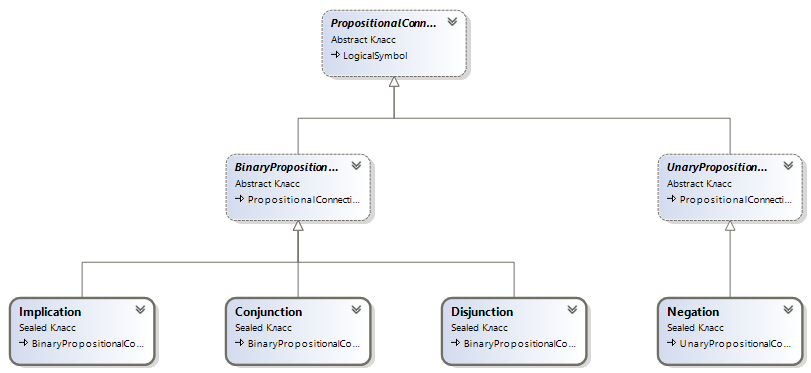
\includegraphics[width=1\linewidth]{PropositionalConnective.png}}
    \caption{Фрагмент диаграммы классов.}
    \label{fig:PropositionalConnective}
\end{figure}

На диаграмме (рис. \ref{fig:PropositionalConnective}), под этим классом, расположены ещё два абстрактных класса для бинарных и унарных связок соответственно. В алфавите языка элементарной алгебры три бинарных связки, которые называются импликация, конъюнкция и дизъюнкция, и одна унарная связка~--- отрицание. Поэтому на нижнем уровне ровно четыре класса. Вновь каждый из этих классов реализует паттерн одиночка, метод ToString возвращает строку с соответствующим классу символом, и определен приоритет~--- $20$, $30$, $40$ и $50$ соответственно для импликации, дизъюнкции, конъюнкции и отрицания.

\subsubsection{Класс Function}

\begin{wrapfigure}{r}{0.20\textwidth}
    %\vspace{-1cm}
    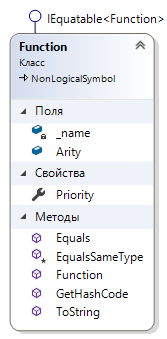
\includegraphics[width=0.9\linewidth]{Function.png}
    \caption{}
    \label{fig:Function}
\end{wrapfigure}

Перейдем к рассмотрению нелогических символов и начнём с класса Function (рис. \ref{fig:Function}), то есть с функциональных символов. Среди членов класса отметим два readonly поля \_name и Arity. Первое из них хранит имя функции (функциональный символ), а второе~--- арность этой функции. Данный класс не является абстрактным, поэтому определено значение приоритета, которое равно $100$. 

На диаграмме (рис. \ref{fig:Function-inh}) видно, что для бинарных операций сложение, вычитание, умножение, деление и возведение в степень реализованы классы Addition, Subtraction, Multiplication, Division и Exponentiation соответственно. Они не являются прямыми потомка класса Function, а для них создан базовый абстрактный класс ArithmeticBinaryFunction. Каждый класс реализует паттерн одиночка и переопределяет значение приоритета:
\begin{itemize}
    \item для сложения и вычитания $110$,
    \item для умножения и деления $120$,
    \item и для возведения в степень $140$.
\end{itemize}

А вот прямым потомком класса Function является класс UnaryMinus, который, очевидно из его имени, описывает унарный минус. Он также реализует паттерн одиночка и переопределяет приоритет, который для него равен $130$.

Таким образом, реализуется <<расширенная версия>> языка элементарной алгебры с дополнительными арифметическими операциями, хотя ранее и было отмечено, что это вовсе необязательно.

\begin{figure}[h]
    \center{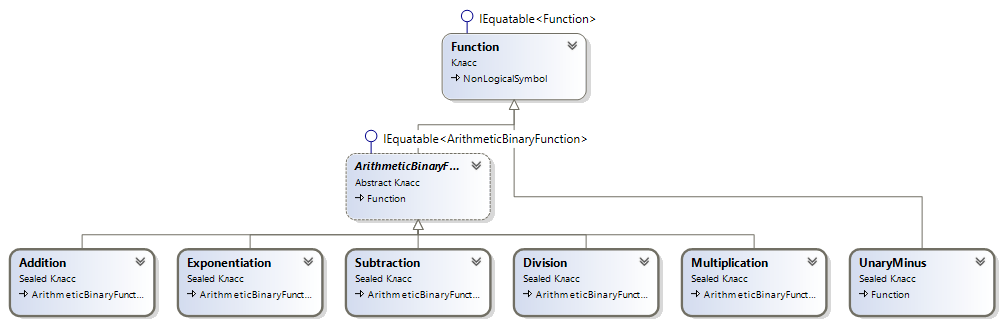
\includegraphics[width=1\linewidth]{Function-inh.png}}
    \caption{Фрагмент диаграммы классов.}
    \label{fig:Function-inh}
\end{figure}

\subsubsection{Класс Predicate}

Класс Predicate схож с классом Function. Также определены поля для имени предиката и для его арности, значение свойства Priority равно $70$. Ниже на диаграмме (рис. \ref{fig:Predicate}) видно два класса-потомка. Оба из них являются абстрактными. Класс ArithmeticPredicate (приоритет равен 80) является базовым для предикатов <<меньше>>, <<равно>> и <<больше>> соответственно, а класс BooleanPredicate (приоритет 90)~--- базовый для \textbf{нульместных} предикатов <<Ложь>> и <<Истина>>.

%\begin{remark}
    Формально, местность (арность) предиката ~--- это натуральное число, но можно считать, что нульместные предикаты~--- это истинностные значения \textbf{И} и \textbf{Л}.
%\end{remark}

\begin{figure}[h]
    \center{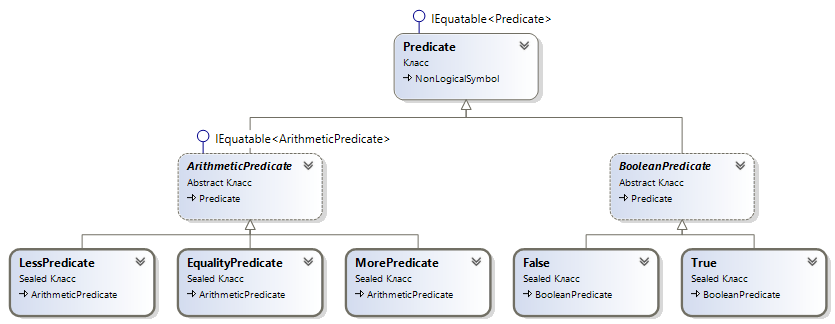
\includegraphics[width=1\linewidth]{Predicate.png}}
    \caption{Фрагмент диаграммы классов.}
    \label{fig:Predicate}
\end{figure}

\subsubsection{Класс IndividualConstant}

Для констант языка написан обобщенный класс IndividualConstant<T> (рис. \ref{fig:Const}), который просто оборачивает тип T. Например, IndividualConstant<int>~--- это целые числа, а рациональные числа записываются как <<целое делить на целое>>. Приоритет констант равен $-10$.

\begin{figure}[h]
    \center{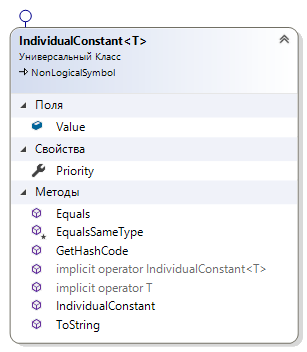
\includegraphics[width=0.3\linewidth]{Const.png}}
    \caption{}
    \label{fig:Const}
\end{figure}

На этом описание классов для символов языка закончено.

\subsubsection{Класс Term}

Прежде чем перейти к описанию формул, необходимо описать класс для термов языка элементарной алгебры. При определении терма выделяется три случая: константа, переменная либо функция от термов. Поэтому абстрактный класс Term является базовым для трех классов (рис. \ref{fig:Term}). Чтобы для формул находить список свободных переменных, объявлено абстрактное свойство FreeObjectVariables, которое очевидным образом реализуют наследники.

\begin{figure}[ht]
    \center{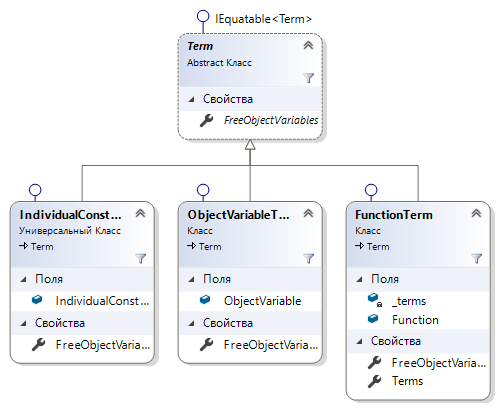
\includegraphics[width=0.5\linewidth]{Term.png}}
    \caption{Фрагмент диаграммы классов.}
    \label{fig:Term}
\end{figure}

Первый и второй классы оборачивают константы и переменные, а третий хранит функцию и массив аргументов, то есть другие термы.

\subsubsection{Класс Formula}

И наконец, объект, для которого были написаны все ранее перечисленные классы~-- формула языка элементарной алгебры. Вновь, исходя из определения формулы получается такая иерархия классов (рис. \ref{fig:Formula}): во главе абстрактный класс Formula и три класса-наследника.

\begin{figure}[h]
    \center{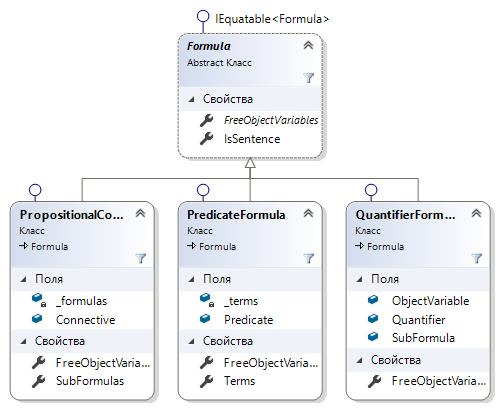
\includegraphics[width=0.5\linewidth]{Formula.png}}
    \caption{Фрагмент диаграммы классов.}
    \label{fig:Formula}
\end{figure}

Класс PredicateFormula описывает формулы вида $p\left(t_1, ... , t_n\right)$, где $p$~-- $n$-местный предикат, а $t_i$~--- терм. Класс PropositionalConnectiveFormula, в котором объявлены поля для пропозициональной связки и аргументов, описывает формулы вида $\mathcal{A} * \mathcal{B}$, где $* \in \left\{\&, \lor, \to\right\}$, или вида $\neg \mathcal{A}$. И для формул вида $(Qx)(\mathcal{A})$ реализован класс QuantifierFormula.

В результате, описаны все объекты языка элементарной алгебры. При этом данная система допускает расширение, например, можно добавлять логические связки, функции или вводить новые предикаты.

\subsection{Система ввода}

Далее необходимо реализовать методы, преобразующие введенную пользователем строку в формулу, то есть в экземпляр класса Formula, или, сообщают о том, что данная строка не является формулой. Аналогичная задача, но для формул исчисления высказываний, была успешно решена в предыдущей работе \cite{Gibadulin1}. В результате, был реализован метод ToFormula класса Parser, в работе которого можно выделить три основных этапа:
\begin{enumerate}
    \item \textbf{лексический анализ}~--- преобразование символов строки в символы алфавита языка элементарной алгебры;
    \item построение \textbf{обратной польской записи};
    \item и \textbf{синтаксический анализ}, в результате которого будет построен экземпляр класса Formula.
\end{enumerate}

Прежде чем перейти к анализу введенной строки, необходимо задать грамматику входного языка:
\begin{equation*}
    \begin{array}{l}
        \begin{array}{ll}
            \text{<формула>} \rightarrow & \left(\text{<формула>}\right) \textbf{|} \\
            & \text{<унарная связка>} \text{<формула>} \textbf{|} \\ 
            & \text{<формула>}\text{<бинарная связка>}\text{<формула>} \textbf{|} \\
            & \text{<терм>}\text{<арифметический предикат>}\text{<терм>} \textbf{|} \\
            & \text{<квантор>}\left(\text{<переменная>},\text{<формула>}\right)
        \end{array} 
        \\
        \begin{array}{ll}
            \text{<унарная связка>} \rightarrow & \text{$\backslash$lnot}
        \end{array} \\   
        \begin{array}{ll}
            \text{<бинарная связка>} \rightarrow & \text{$\backslash$land} \textbf{|}\text{$\backslash$lor} \textbf{|} \text{$\backslash$to}
        \end{array} \\  
        \begin{array}{ll}
            \text{<арифметический предикат>} \rightarrow & $<$\textbf{|}$>$\textbf{|}$=$
        \end{array} \\ 
        \begin{array}{ll}
            \text{<квантор>} \rightarrow & \text{$\backslash$exists} \textbf{|} \text{$\backslash$forall}
        \end{array} \\  
        \begin{array}{ll}
            \text{<переменная>} \rightarrow & \text{<буква>} \textbf{|} \text{<буква>\_<натуральное число>}
        \end{array} \\  
        \begin{array}{ll}
            \text{<терм>} \rightarrow & \left(\text{<терм>}\right) \textbf{|} \\
            & \text{<переменная>} \textbf{|} \\ 
            & \text{<натуральное число>} \textbf{|} \\
            & \text{<унарный минус>}\text{<терм>} \textbf{|} \\
            & \text{<терм>}\text{<арифметическая функция>}\text{<терм>} \textbf{|} \\
            & \text{<терм>}\text{<возведение в степень>}\text{<натуральное число>}\\
        \end{array} 
        \\
        \begin{array}{ll}
            \text{<унарный минус>}\rightarrow & -
        \end{array} \\ 
        \begin{array}{ll}
            \text{<арифметическая функция>}\rightarrow & + \textbf{|} - \textbf{|} * \textbf{|} / \textbf{|} \backslash \text{over}
        \end{array} \\ 
        \begin{array}{ll}
            \text{<возведение в степень>}\rightarrow & \wedge
        \end{array}
    \end{array}       
\end{equation*}

%\begin{remark}
    Нетерминальные символы <натуральное число> и <буква> определяются стандартным образом.
%\end{remark}

%\begin{remark}
    При реализации была заложена возможность вводить функции и предикаты с произвольным именем и с произвольной арностью (местностью), но в грамматике это не отражено, так как данный механизм далее никак не используется.
%\end{remark}

На этапе лексического анализа входная строка разбивается на терминальные символы (лексемы, токены), в нашем случае, на объекты класса Symbol, пробелы опускаются. Если обнаружен символ, который не принадлежит алфавиту, то генерируется сообщение об ошибке с указанием неопознанного символа и его индекса во входной строке. Все выше перечисленное реализовано в методе ToSymbols класса Parser. А также в этом методе реализован механизм, который отличает унарный минус от бинарного.

Далее, вызовом метода ToRpn, строится обратная польская запись последовательности символов алгоритмом Дейкстры. Этот алгоритм просматривает список входных символов. В зависимости от приоритета символ либо сразу помещается в выходную последовательность (отрицательный приоритет), либо выталкивает из стека символы с большим приоритетом, после чего сам заносится в стек. При этом метод ToRpn производит ряд простых проверок расположения символов в строке, например, две переменные не могут идти друг за другом.

И наконец, по правилам грамматики <<вычисляется>> формула, объект класса Formula, таким же способом как происходит вычисление арифметического выражения, записанного в виде обратной польской записи. Именно на этом этапе обнаруживается большинство ошибок, для каждой из которых генерируется сообщение об ошибке.

\subsection{Реализация алгоритма Тарского}

Переходим непосредственно к реализации алгоритма построения бескванторной формулы, а точнее к рассмотрению библиотеки SimpleTarskiAlgorithmLib.

Первым делом рассмотрим перечисление Sign, так как именно знаки чисел и многочленов являются важной и при этом самой простой частью алгоритма. В этом перечислении определены следующие значения:
\begin{itemize}
    \item NotNumber~--- объект не имеет знака;
    \item LessZero~--- меньше нуля;
    \item MoreZero~--- больше нуля;
    \item Zero~--- нуль;
    \item NotMoreZero~--- не больше нуля;
    \item NotLessZero~--- не меньше нуля;
    \item NotZero~--- не нуль; 
    \item Undefined~--- знак может быть любым.
\end{itemize}

Так как рассматриваются многочлены с коэффициентами из $\mathbb{Q}$, необходимо реализовать структуру для рациональных чисел. Для этого достаточно в качестве целых чисел взять структуру BigInteger и вспомнить как определяются рациональные числа и операции над ними в алгебре. Поэтому для этой структуры определены поля для числителя и знаменателя, а также поле для знака числа. Естественным образом реализованы арифметические операции сложение, вычитание, умножение, деление и возведение в натуральную степень.

Для реализации класса для многочленов вновь необходимо вспомнить как они определяются в алгебре и реализовать эти определения в виде программы. Поэтому в классе Polynomial определен массив из рациональных чисел, переменная типа VariableName и поля для знака многочлена. Как в алгебре старший коэффициент многочлена отличен от нуля, так и элемент массива с наибольшим индексом не должен быть равным нулю. Для многочленов определены операции сложения, вычитания, умножения, деление с остатком, формальное дифференцирование и возведение в натуральную степень.

Переходим к задаче насыщения системы многочленов. Для её решения создан статический класс SimpleSaturator, а точнее его метод Saturate. На вход ему поступает последовательность многочленов. Затем он из них выбирает все ненулевые, вычисляет производную их произведения и помещает выбранные многочлены и производную в очередь. Далее пока очередь не пуста происходит следующее:
\begin{itemize}
    \item Извлекаем из очереди первый многочлен $P$. Если он уже добавлен в результирующее множество, то есть в HashSet<Polynomial>, то переходим к следующей итерации цикла;
    \item Добавляем в очередь производную этого многочлена;
    \item Для каждого многочлена $Q$ из результирующего множества добавляем его остаток от деления на $P$, если $deg(Q) \geq deg(P)$, и остаток от деления $P$ на $Q$, если $deg(P) \geq deg(Q)$.
\end{itemize} 

После этапа насыщения системы следует этап построения таблицы Тарского, поэтому необходимо реализовать структуру данных соответствующую свойствам таблицы. Во-первых, довольно часто будут добавляться столбцы, поэтому предлагается рассматривать таблицы как связный список столбцов, что позволяет наиболее эффективно добавлять новые столбцы. Во-вторых, строки добавляются только в конец таблицы, поэтому столбцы представляют собой список знаков~--- List<Sign>, так как добавление в конец списка и обращение к элементу списка происходят достаточно быстро.

Рассмотрим последнюю библиотеку~--- SimpleTarskiAlgorithmRunner. Именно класс SimpleTarskiAlgorithm, расположенный в этой библиотеке, связывает формулы и алгоритм Тарского. QuantifiersElimination~--- единственный публичный метод этого класса. Он реализует алгоритм $B$, описанный в утверждении \ref{algB}, а алгоритм $A$, то есть алгоритм Тарского для формулы вида $(Qx)\Phi(x)$, реализован в виде метода TarskiEliminate.

На этом заканчивается описание программы. Исходный код проекта размещен в виде репозитория на GitHub, ссылку на который можно найти в приложении А. Еще в репозитории можно найти проекты с юнит-тестами, так как весь код отлаживался, а наиболее сложные его части тестировались.

\subsection{Демонстрация работы}

Чтобы продемонстрировать работу программы было создано простое консольное приложение. Пользователю предлагается ввести формулу. После того как пользователь ввел формулу ему выводится сообщение о том, в какой файл записан результат работы программы. Далее (рис. \ref{fig:примеры}) приведено несколько примеров содержания таких выходных файлов.

Для того, чтобы реализовать алгоритм Тарского для формул общего вида, необходимо, во-первых, реализовать многочлены с параметрами, во-вторых, насыщение системы. Если с многочленами сложностей не возникает (в проекте уже реализован соответствующий класс), то насыщение системы таких многочленов оказалось нетривиальной задачей, так как требует разбора случаев знака коэффициентов. При этом построение таблицы и остальные части, за редким исключением, не отличаются от того, что уже было реализовано. Поэтому можно сказать, что в данной работе реализован базовый, но наиболее важный и трудоёмкий случай.


\begin{figure}[ht]
    \begin{minipage}[ht]{0.349\linewidth}
        \center{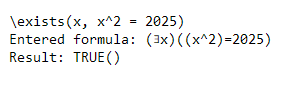
\includegraphics[width=0.99\linewidth]{пример1.PNG} \\ а)}
    \end{minipage}
    \hfill
    \begin{minipage}[ht]{0.65\linewidth}
        \center{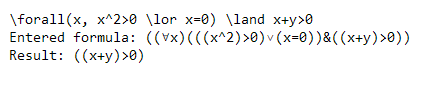
\includegraphics[width=0.99\linewidth]{пример2.PNG} \\ б)}
    \end{minipage}
    \\
    \begin{center}
        \begin{minipage}[ht]{0.8\linewidth}
            \center{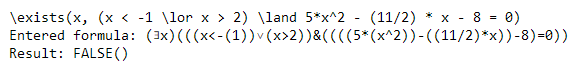
\includegraphics[width=0.99\linewidth]{пример3.PNG} \\ в)}
        \end{minipage} 
    \end{center}
    \caption{Примеры выходных данных.}  
    \label{fig:примеры}
\end{figure}